% Made up for the tikra benchmark.
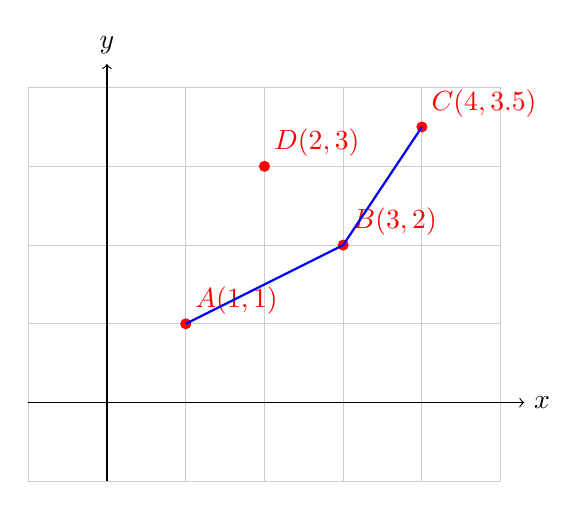
\begin{tikzpicture}
  \draw[step=1, gray!40] (-1,-1) grid (5,4);
  \draw[->] (-1,0) -- (5.3,0) node[right] {$x$};
  \draw[->] (0,-1) -- (0,4.3) node[above] {$y$};
  \foreach \x/\y/\n in {1/1/A, 3/2/B, 4/3.5/C, 2/3/D} {
    \fill[red] (\x,\y) circle (2pt) node[above right] {$\n(\x,\y)$};
  }
  \draw[blue, thick] (1,1) -- (3,2) -- (4,3.5);
\end{tikzpicture}
